\documentclass[11 pt]{article}
\usepackage[bmargin=1in,tmargin=1in,lmargin=0.75in,rmargin=0.75in]{geometry}
\usepackage[dvipsnames]{xcolor}
\usepackage{amsfonts,amsmath,amsthm,color,amssymb, url, enumerate, bbm}
\usepackage{pgfplotstable, pgfplots}
\usepackage{graphicx}
\usepackage{tikz}
\usetikzlibrary{patterns, arrows}
\usepackage{subcaption}
\usepackage[noend]{algpseudocode}
\usepackage{algorithm}
\usepackage{float}
\usepackage[bottom]{footmisc}
\usepackage{mathptmx}
\usepackage[11pt]{moresize}

\usepackage{hyperref}
\hypersetup{
    colorlinks=true,
    linkcolor=blue,
    filecolor=blue,      
    urlcolor=blue,
}

\iffalse
\usepackage{fancyhdr}
\pagestyle{fancy}
\fancyhf{}
\rhead{}
\lhead{}
\fi

\newcommand{\code}[1]{\colorbox{gray!10}{\textcolor{black!85}{\texttt{#1}}}}

\title{Introduction to Google OR-Tools for ENGRI 1101 \footnote{Currently set up for use by course developers. Should be updated and reworked for 1101 students.}}

\begin{document}
\date{}

\maketitle

\section{Installation}

The quickest way to get OR-Tools working for Python is to \href{https://developers.google.com/optimization/install}{install the binary version}. This can be done by running the following in terminal:
$$\code{python -m pip install --upgrade --user ortools}$$
However, to use OR-Tools with a third-party solver (such as Gurobi), it must be compiled from source. Google offers reasonably detailed instructions on doing so for \href{https://developers.google.com/optimization/install/python/source_linux}{Linux}, \href{https://developers.google.com/optimization/install/python/source_mac}{MacOS}, and \href{https://developers.google.com/optimization/install/python/source_windows}{Windows}. However, some additional steps may be necessary. Here, we give a full set of instructions to successfully use Gurobi through OR-Tools on both MacOS and Windows. \newline

\subsection{Windows}
These instructions are adapted from those presented by David Williamson and Jody Zhu.
\begin{enumerate}
\item Install \href{https://visualstudio.microsoft.com/downloads/}{Visual Studio 2019 Community} and Build Tools for Visual Studio 2019. Your Visual Studio Installer should look like this:
\begin{center}
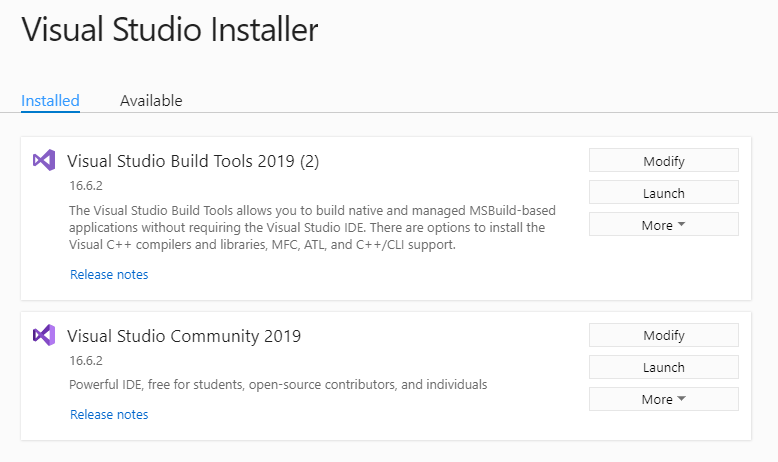
\includegraphics[scale=0.4]{VS.png}
\end{center}
\item Click ``Modify" for Build Tools. Then check ``C++ build tools."
\begin{center}
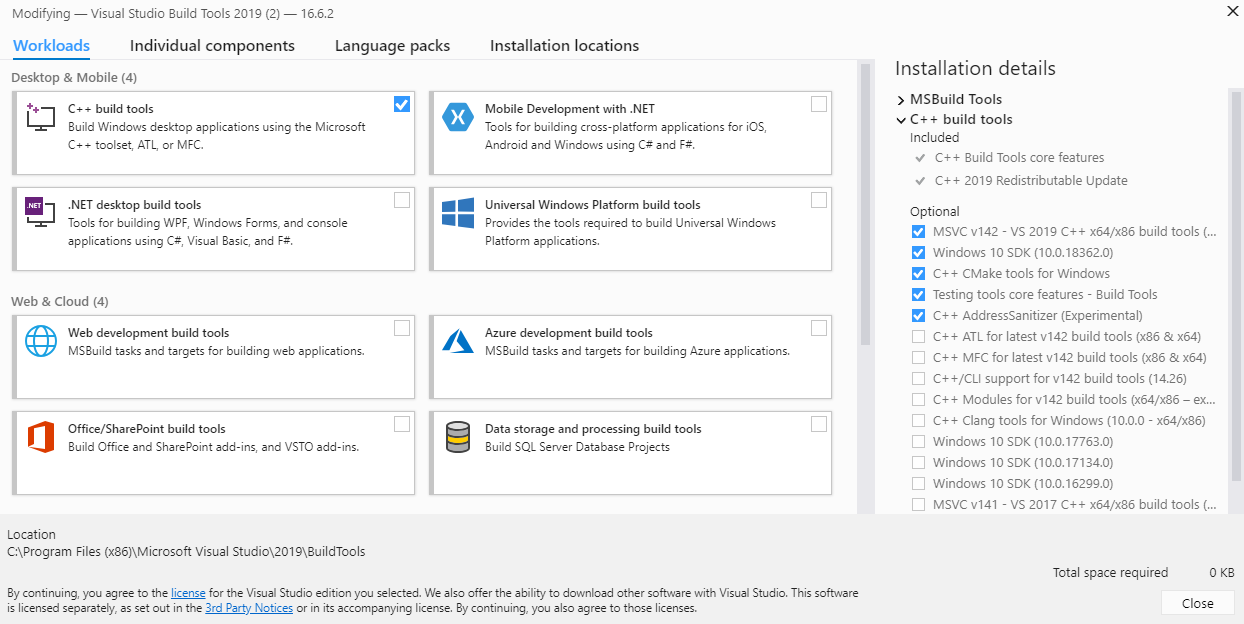
\includegraphics[scale=0.3]{Modify.png}
\end{center}
\item Install \href{https://www.cmake.org/download}{cmake} using ``Windows win64-x64 Installer" under Binary distributions.
\item Make sure you have the correct Python and Git.
\item Run \code{git clone -b master https://github.com/google/or-tools} to get the master branch of the source code (Any command prompt can be used here which is \textbf{not} the case for the next step).
\item Open x64 Native Tools Command Prompt that is in the Visual Studio 2019 folder
\begin{center}
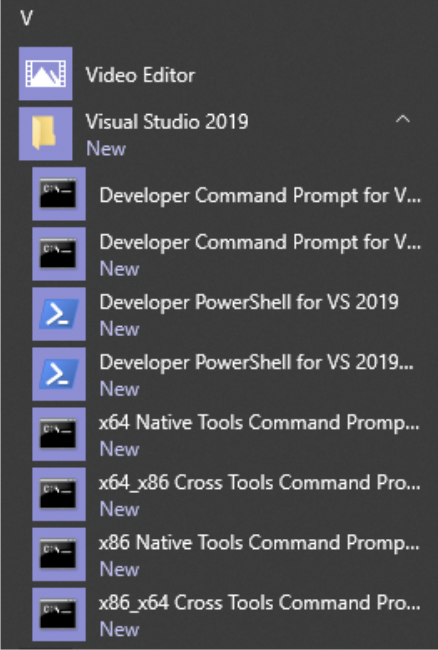
\includegraphics[scale=0.5]{NativeToolsCommandPrompt.png}
\end{center}
\item Navigate to your ``or-tools" folder (cd .. to go up and cd ``name" to go down)
\item Run \code{tools\textbackslash make third\_party}
\item \textit{(Assumes Gurobi has been installed correctly with a license)} Edit the \texttt{Makefile.local} file. Note that \texttt{WINDOWS\_GUROBI\_DIR} might be different depending where ``gurobi902" is located. 
\begin{center}
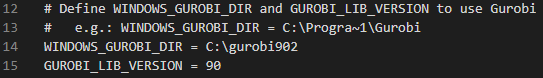
\includegraphics[scale=0.6]{MakefileLocal.png}
\end{center}
\item Run \code{tools\textbackslash make python}
\item This stopped with an error for me, so I edited \texttt{Makefile.win.mk} on the line for \texttt{STATIC\_SCIP\_LNK} to change \texttt{scip.lib} to \texttt{libscip.lib}.  Then I reran \code{tools\textbackslash make python}, and this worked.
\item I need to install a package wheel, so ran \code{pip install wheel}
\item Run \code{tools\textbackslash make install\_python}
\item If you previously installed ortools from binary, run \code{pip uninstall ortools}
\end{enumerate}

\subsection{MacOS}
These instructions are adapted from those presented by David Williamson
\begin{enumerate}
\item Run \code{xcode-select --install} 
\item Verify \code{xcode-select -p} returns \code{/Applications/Xcode.app/Contents/Developer}
\item Install Homebrew: \newline
\begin{small} \code{/usr/bin/ruby -e "\$(curl -fsSL https://raw.githubusercontent.com/Homebrew/install/master/install)"} \end{small}
\item Update Homebrew: \code{brew update}
\item Verify \code{brew --version} returns \newline
\code{Homebrew 1.6.9-8-g25542d7} \newline
\code{Homebrew/homebrew-core (git revision 0e0c84; last commit 2018-06-20)}
\item Install the remaining prerequisites:
\begin{enumerate}
\item Run \code{brew install cmake wget pkg-config}
\item Run \code{brew install swig}
\item Run \code{brew install python}
\item Run \code{python3 -m pip install -U --user wheel six}
\end{enumerate} 
\item Run \code{git clone -b master https://github.com/google/or-tools} to get the source master branch
\item Navigate to installation location
\item Run \code{make third\_party}
\item \textit{(Assumes Gurobi has been installed correctly with a license)} Edit the \texttt{Makefile.local} file. Note that \texttt{UNIX\_GUROBI\_DIR} might be different depending where ``gurobi902" is located. 
\begin{center}
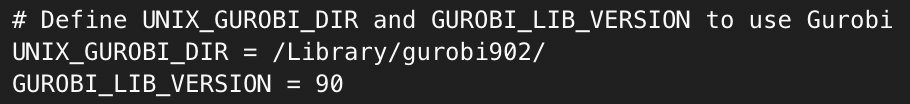
\includegraphics[scale=0.7]{MakefileMac.png}
\end{center}
\item Run \code{make python}
\item Run \code{make install\_python}
\item You may have to edit a line in in \texttt{makefiles\textbackslash Makefile.python.mx} by adding \texttt{--prefix=} at the end 
\begin{center}
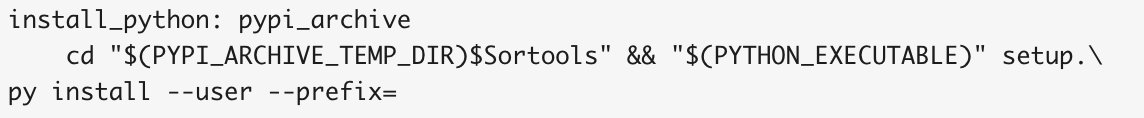
\includegraphics[scale=0.7]{MakefileLastStep.png}
\end{center}
\item If you previously installed ortools from binary, run \code{pip uninstall ortools}
\end{enumerate} 

\section{Documentation}

Google offers decent \href{https://developers.google.com/optimization/reference/python/linear_solver/pywraplp}{documentation}. Here, we introduce the subset of functionality that 1101 students will use. Furthermore, some standard style guidelines are established\footnote{Style guidelines are adapted from those written by Jody Zhu}.

\subsection{Imports}

All Jupyter Notebooks should begin with the following imports named accordingly. Both \texttt{numpy} and \texttt{math} are standard imports. \texttt{pandas} is used for manipulating CSV files which act as AMPL dat files. \texttt{itertools} is used for taking the cartesian product of two or more sets. Lastly, \texttt{pywraplp} is the package used for creating and solving LPs.
\begin{center}
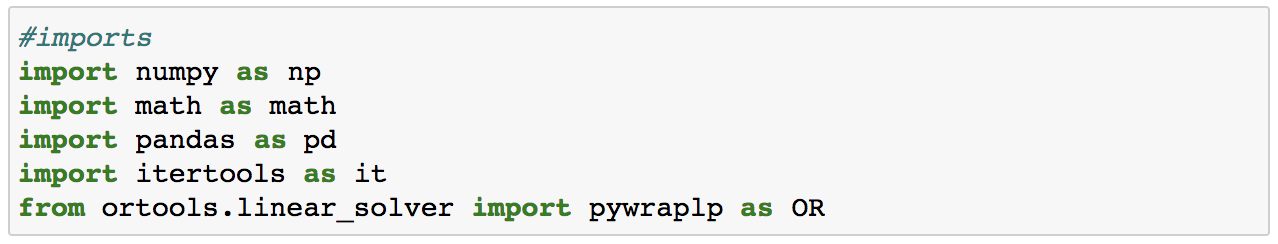
\includegraphics[scale=0.7]{imports.png}
\end{center}

\subsection{Model}

To solve an LP or MIP, we first create a \texttt{Solver} similar to an AMPL model. $$\code{m = OR.Solver(<name>, <problem\_type>)}$$ instantiates a solver where \texttt{problem\_type} declares which solver is used to solve the model. Assuming OR-Tools was complied from source for use with Gurobi, the available options for \texttt{problem\_type} are
\begin{itemize}
\item \texttt{GLOP\_LINEAR\_PROGRAMMING}: An open-source LP solver (by Google)
\item \texttt{CBC\_MIXED\_INTEGER\_PROGRAMMING}: An \href{https://github.com/coin-or/Cbc}{open-sorce} MIP solver
\item \texttt{GUROBI\_MIXED\_INTEGER\_PROGRAMMING}: A leading commercial MIP solver
\end{itemize}
For example, we can define a model named ``ex" that uses Gurobi to solve mixed integer programs:
\begin{center}
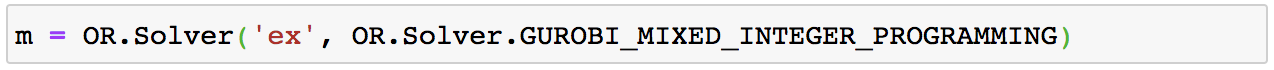
\includegraphics[scale=0.7]{model.png}
\end{center}
Use \code{m.EnableOutput()} to see solver output. \textcolor{red}{(This goes to terminal right now. Looking into a better way)}

\subsection{Sets and Parameters}

Similar to AMPL, sets should be named in uppercase. In Python, they are represented by a list. Some helpful commands are \code{SET.append(x)} which adds \texttt{x} to the \texttt{SET} and \code{SET1.extend(SET2)} which adds elements of \texttt{SET2} to \texttt{SET1}. Furthermore, \code{list(it.product(SET1,SET2))} returns the cartesian product of \texttt{SET1} and \texttt{SET2}. Parameters should be named in lowercase. It is good practice to keep both set and parameter names no more than 6 characters. Parameters that have values for every element of a set should be stored as a Python dictionary. Here is an example for a max flow formulation (which will serve as a running example).
\begin{center}
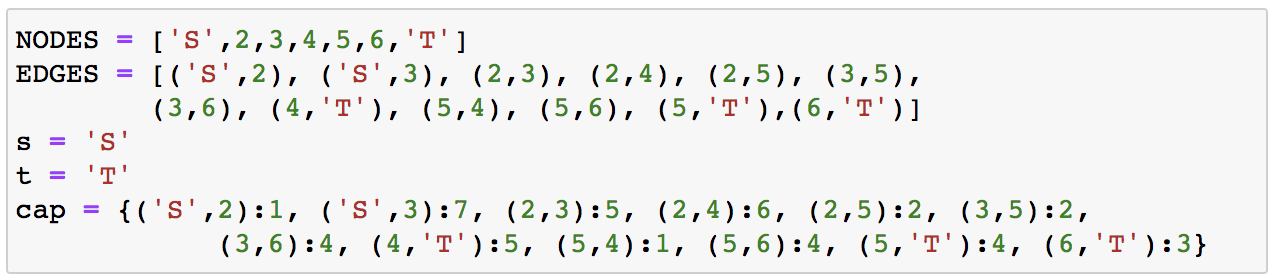
\includegraphics[scale=0.7]{setAndParam.png}
\end{center}

\subsection{Variables}

To add an additional variable to a model, we use the method \code{m.NumVar(<lb>, <ub>, <name>)} for continuous variables and \code{m.IntVar(<lb>, <ub>, <name>)} for integer variables. In both cases, \texttt{lb} and \texttt{ub} refer to the lower and upper bound for that variables respectively. Note that \texttt{m.infinity()} and \texttt{-m.infinity()} can be used when there is no upper or lower bound. The decision variables for the max flow formulation are instantiated as follows.
\begin{center}
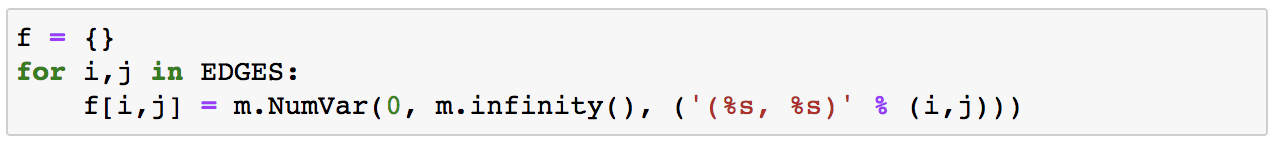
\includegraphics[scale=0.7]{var.png}
\end{center}

\subsection{Objective Function}

The objective function is specified by passing an expression in the variables to \code{m.Maximize(<expression>)} or \code{Minimize(<expression>)} depending on the direction of optimization. Often, expressions consist of a summation. In Python, \code{sum(x[i] for i in SET if <boolean expression>)} is useful for summing over elements. The objective of max flow is
\begin{center}
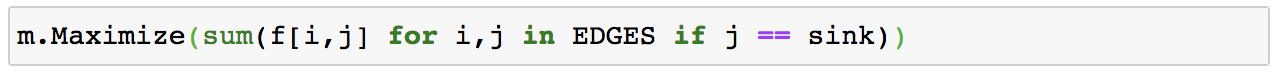
\includegraphics[scale=0.7]{obj.png}
\end{center}

\subsection{Constraints}

To add a constraint to the model, we use \code{m.Add(<boolean expression>)} where the constraint is represented by some boolean expression in the variables. The only comparison operators that should be used are \texttt{<=}, \texttt{>=}, or \texttt{==}. It is best practice to have some comment describing what each constraint does as seen below.
\begin{center}
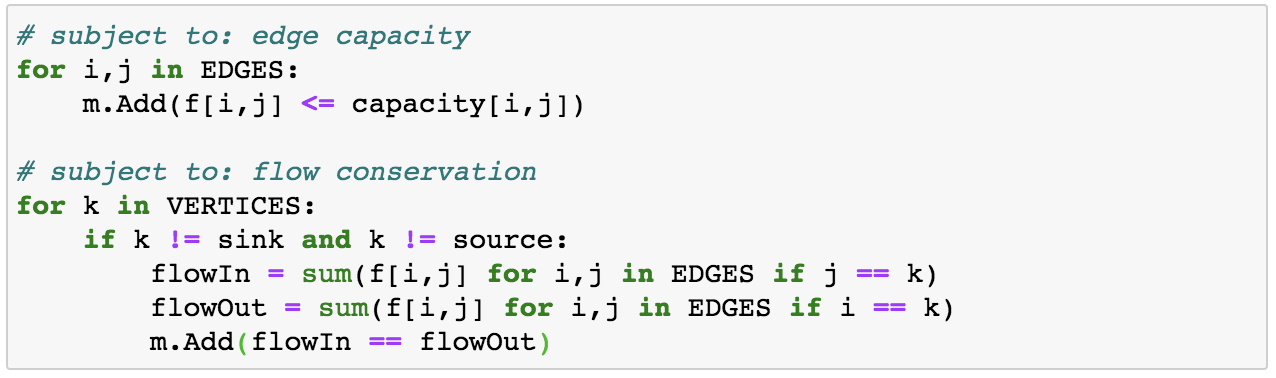
\includegraphics[scale=0.7]{constraints.png}
\end{center}

\subsection{Solve}

To solve the model, we use \code{m.Solve()}. The optimal value is then retrieved using \code{m.Objective().Value()}. By iterating through \code{m.variables()}, one can examine the value of each variable using method \code{.solution\_value()}. An example solution output is:
\begin{center}
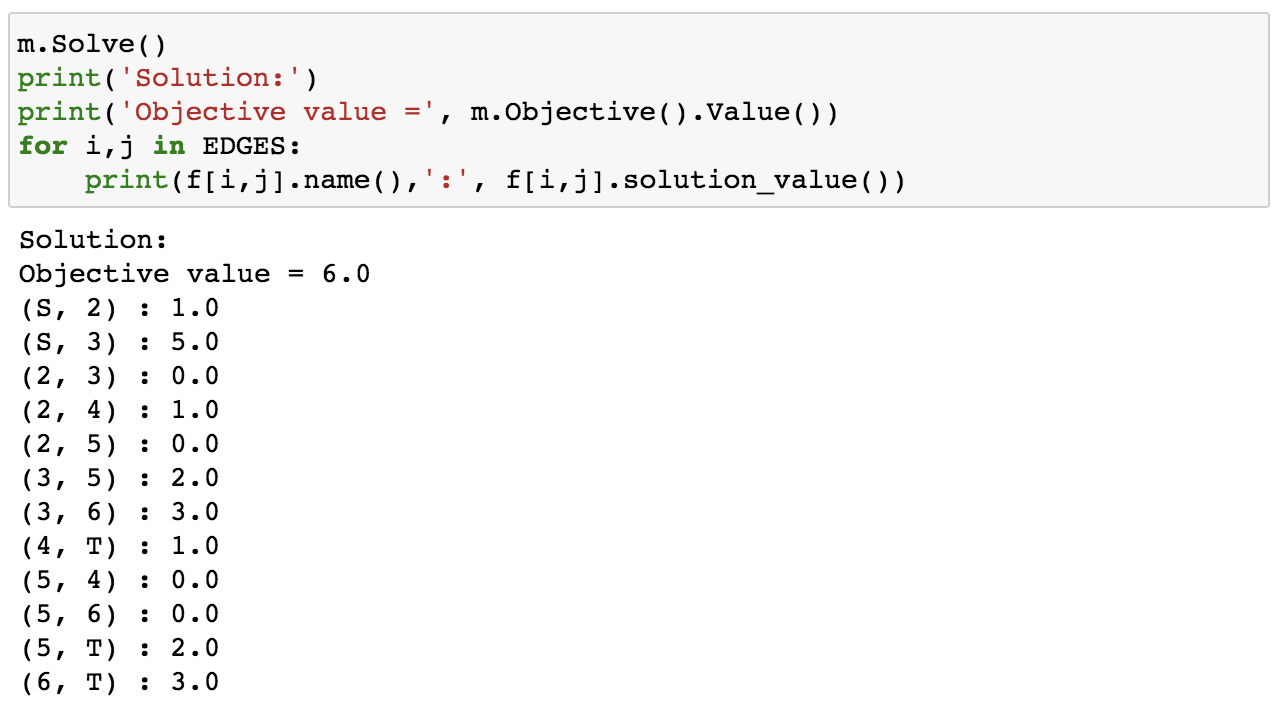
\includegraphics[scale=0.7]{sol.png}
\end{center}

\subsection{Early Termination}

One way to terminate early is by setting a time limit. This can be done using \code{m.SetTimeLimit(<time>)} where \texttt{<time>} is the time limit in milliseconds. For MIPs, one can terminate by the relative MIP gap defined as 
$$\frac{|\texttt{best\_bound} - \texttt{incumbent}|}{|\texttt{incumbent}|}.$$
This is done as follows: 
\begin{center}
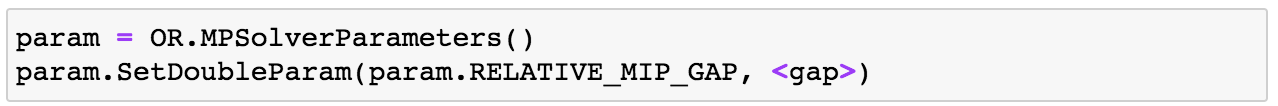
\includegraphics[scale=0.7]{gap.png}
\end{center}
where \texttt{<gap>} is the gap to terminate at (say 0.05 for a solution within 5\% of optimal). Note, when running \code{m.Solve()}, you must pass these parameters using \code{m.Solve(param)}. If one terminates by time limit, the MIP gap can be ascertained through
\begin{center}
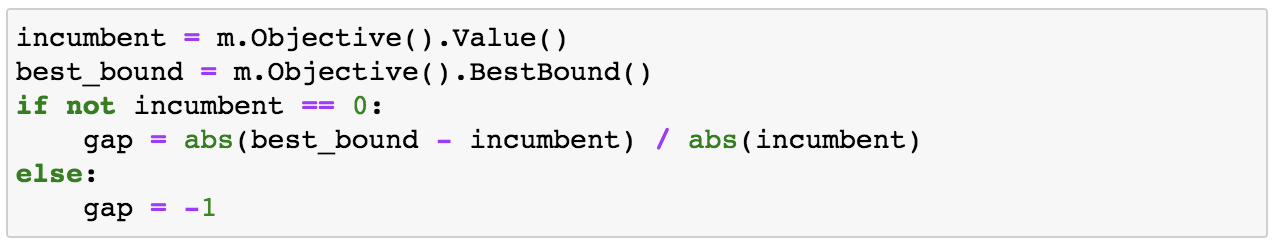
\includegraphics[scale=0.7]{gapDef.png}
\end{center}
If the time limit is set too small, the solver may not reach a feasible solution. In this case, every variable is set to zero. This often results in an objective value of zero. Hence, to prevent a divide by zero error when dividing by the incumbent, the gap is set to -1 \textcolor{red}{(may be better ways to handle this...)}

\subsection{Solver-Specific Parameters}

Gurobi offers an extensive set of \href{https://www.gurobi.com/documentation/9.0/refman/parameters.html}{parameters} that ``control the operation of the Gurobi solver." All of these parameters can be set through the OR-Tools interface using \code{m.SetSolverSpecificParametersAsString(<param\_file>)} where \texttt{param\_file} is a \href{https://www.gurobi.com/documentation/9.0/refman/prm_format.html#format:PRM}{PRM file}. Below is an example of some possible termination parameters that could be set.

\begin{center}
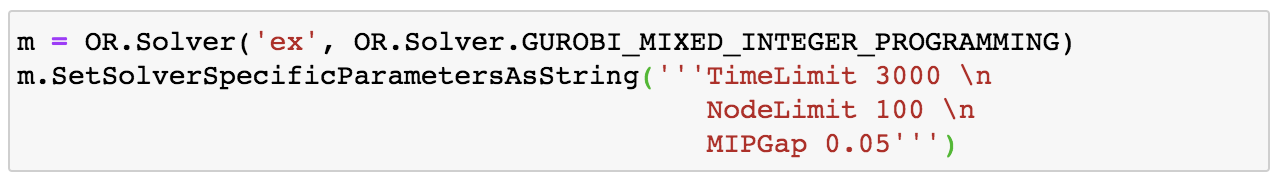
\includegraphics[scale=0.7]{Gparams.png}
\end{center}

\textcolor{red}{(To my knowledge, one can not set general parameters for CBC yet)}


\end{document}











